\usecaseristoratore{Visualizzazione lista prenotazioni}
\label{usecase:Visualizzazione lista prenotazioni}

\begin{figure}[h]
	\centering
	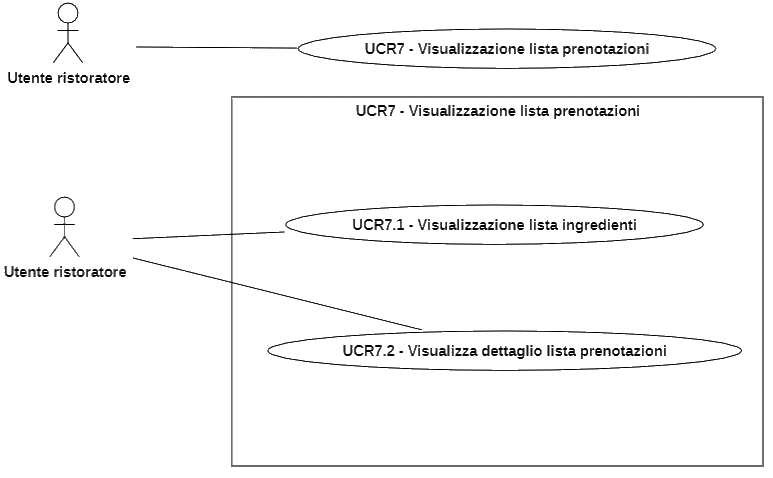
\includegraphics[width=0.999\textwidth]{./uml/UCR7.png} 
	\caption{Visualizzazione lista prenotazioni}
	\label{fig:UCR7}
  \end{figure}

\begin{itemize}
	\item \textbf{Attore principale:} Utente ristoratore.

	\item \textbf{Precondizione:} L'Utente ristoratore ha effettuato l'accesso al Sistema (vedi \autoref{usecase:Effettua accesso}).

	\item \textbf{Postcondizione:} L'Utente ristoratore visualizza la lista di prenotazioni (prenotazioni che si trovano in qualsiasi stato) attraverso una vista a calendario settimanale.

	\item \textbf{Scenario principale:}
	      \begin{enumerate}
		      \item Il Sistema mostra una vista a calendario settimanale, in ogni giorno della settimana l'utente può consultare:
		            \begin{itemize}
			            \item La lista di prenotazioni.
			            \item La lista di ingredienti con le quantità necessarie per soddisfare la richiesta giornaliera (vedi \autoref{usecase:Consultazione lista ingredienti}).
		            \end{itemize}

		      \item Il Sistema mostra la lista prenotazioni inerente ad un giorno nei due modi seguenti:
		            \begin{itemize}
			            \item Di \textit{default}, nella lista, le prenotazioni che vengono mostrate per prime sono quelle che si trovano nello stato "Accettata".

			            \item L'Utente ristoratore può applicare un filtro basato sullo stato della prenotazione, per facilitare la consultazione della lista a seconda dei suoi bisogni.
		            \end{itemize}

		      \item L'Utente ristoratore visualizza la lista di prenotazioni a vista settimanale.
	      \end{enumerate}
\end{itemize}


\subusecaseristoratore{Visualizzazione lista ingredienti}
\label{usecase:Consultazione lista ingredienti}
\begin{itemize}

	\item \textbf{Attore principale:} Utente ristoratore.

	\item \textbf{Precondizione:} L'Utente ristoratore si trova nella sezione "Consultazione lista prenotazioni" (vedi \autoref{usecase:Visualizzazione lista prenotazioni}).

	\item \textbf{Postcondizione:} L'Utente ristoratore visualizza la lista ingredienti aggiornata.

	\item \textbf{Scenario principale:}
	      \begin{enumerate}
		      \item Il Sistema mostra la lista ingredienti necessari per la giornata (relativamente alle prenotazioni nello stato "Accettata");
		      \item L'Utente ristoratore visualizza la lista degli ingredienti.
	      \end{enumerate}

\end{itemize}

\subusecaseristoratore{Visualizza dettaglio lista prenotazioni}
\label{usecase:Visualizza dettaglio lista prenotazioni}
\begin{itemize}
	\item \textbf{Attore principale:} Utente ristoratore.

	\item \textbf{Precondizione:} L'Utente ristoratore ha consultato la lista delle prenotazioni (vedi \autoref{usecase:Visualizzazione lista prenotazioni}).

	\item \textbf{Postcondizione:} L'Utente ristoratore visualizza le prenotazioni in dettaglio.


	\item \textbf{Scenario principale:}
	      \begin{enumerate}
		      \item L'Utente ristoratore seleziona un giorno nel calendario a vista settimanale da visualizzare in dettaglio;
		      \item Il Sistema mostra tutte le prenotazioni presenti nel giorno selezionato dall'Utente ristoratore;

		      \item L'Utente ristoratore seleziona una prenotazione da visualizzare in dettaglio;
		      \item Il Sistema mostra i dettagli e le informazioni relative alla prenotazione selezionata dall'Utente ristoratore:
		            \begin{itemize}
			            \item Nome collegato alla prenotazione.
			            \item Numero di persone.
			            \item Stato della prenotazione.
			            \item Giorno e l'orario della prenotazione.
			            \item Eventuali persone con difficoltà motoria.
		            \end{itemize}

	      \end{enumerate}
\end{itemize}
